\documentclass{article}

\usepackage[main, final]{neurips_2026}

\usepackage[utf8]{inputenc}
\usepackage[T1]{fontenc}
\usepackage{hyperref}
\usepackage{url}
\usepackage{booktabs}
\usepackage{amsfonts}
\usepackage{amsmath}
\usepackage{amssymb}
\usepackage{microtype}
\usepackage{xcolor}
\usepackage{graphicx}
\usepackage[section]{placeins}
\usepackage{float}
\usepackage{cleveref}

\makeatletter\renewcommand{\@notice}{}\makeatother
\makeatletter\setlength{\@fptop}{0pt}\makeatother

\newcommand{\tablebody}[1]{\small\setlength{\tabcolsep}{4pt}\input{#1}}
\newcommand{\apptable}[1]{\footnotesize\setlength{\tabcolsep}{3pt}\input{#1}}

\renewcommand{\topfraction}{0.9}
\renewcommand{\bottomfraction}{0.6}
\renewcommand{\textfraction}{0.07}
\renewcommand{\floatpagefraction}{0.85}

\title{Adaptation, Visual Grounding and Test-Time Compute\\in Small Language Models}

\author{%
  Abdul Hafeez \\
  Advanced Topics in Machine Learning, Fall 2026\\
  \texttt{25280098@lums.edu.pk}
}

\begin{document}

\maketitle

\begin{abstract}
Adapting a pretrained language model aims to improve a target task without lowering its performance on other tasks. However, each adaptation optimizes a proxy that can diverge from this goal, such as cross-entropy on a narrow dataset or on captions, or agreement among sampled answers. We fine-tune Qwen3-0.6B on mathematics with full updates, an L2 penalty toward the starting weights (L2-SP), Low-Rank Adaptation (LoRA) and orthogonally projected LoRA (OPLoRA). We also train a three-stage SigLIP--Qwen3 vision-language model (VLM), and select answers among repeated samples of Qwen2.5 models with adaptive stopping. Because the loss covers every response token, full fine-tuning learned the closing line of its training answers and inserted it into unrelated conversations, which likelihood benchmarks never test. OPLoRA matched LoRA because LoRA's updates already placed no more of their energy in the protected singular directions than a random update would. The VLM's answers depended on the image only after training on answers that change with the image. Majority voting missed correct answers given by a minority of rollouts, and model confidence raised accuracy as a vote weight but lowered it as a single-rollout selector. \href{https://github.com/hafeez381/llm-adaptation}{Code}.
\end{abstract}

\section{Introduction}
\label{sec:intro}

A pretrained language model with parameters $\theta_0$ defines a distribution $p_{\theta_0}(y\mid x)$ over responses $y$ to a prompt $x$, and adapting it means changing what it produces on a target task without lowering its performance on other tasks. Fine-tuning changes the parameters by solving
\begin{equation}
\label{eq:ft}
\min_\theta\; L_{\mathrm{SFT}}(\theta)+\lambda\,\Omega(\theta,\theta_0)\quad\text{subject to}\quad\theta-\theta_0\in S,
\end{equation}
where $L_{\mathrm{SFT}}$ is the supervised fine-tuning (SFT) loss, i.e.\ the token-averaged cross-entropy on target responses, $\Omega$ penalizes distance from $\theta_0$ with strength $\lambda$, and $S$ is the set of allowed updates. A modular vision-language model (VLM) keeps the language model frozen and prefixes the text with visual tokens from a trainable image connector, allowing $p_\theta(y\mid I,x)$ to condition on the image. Test-time compute keeps model parameters fixed and samples multiple rollouts from $p_\theta(y\mid x)$, selecting a final answer through voting or scoring rules. For each adaptation we ask what it changed besides its target, and whether its loss or selection rule explains the change. We study how five fine-tuning methods balance mathematical gains against other capabilities (\Cref{sec:t1}), when a VLM's answers come to depend on the correct image (\Cref{sec:t2}), and how repeated sampling, answer selection and adaptive stopping turn extra generation into accuracy (\Cref{sec:t3}).

\section{Experimental Setup}
\label{sec:setup}
\paragraph{Models and Training.} Every run started from a released checkpoint with seed 6304 on one NVIDIA T4 GPU, with the thinking mode of Qwen3 disabled. Training used FP16 mixed precision with 32-bit copies of the trainable weights (Appendix~\ref{app:dev}). Fine-tuned models were evaluated zero-shot in FP16 with the lm-evaluation-harness \citep{lmeval}. Leakage guards and deviations are in Appendix~\ref{app:dev}.

\section{Language Model Fine-Tuning}
\label{sec:t1}
\subsection{Setup}
\paragraph{Methods.} The five fine-tuning methods are instances of \Cref{eq:ft}. Full fine-tuning (Full FT) updates every parameter with $\lambda=0$. Full FT + L2-SP adds $\Omega=\tfrac12\lVert\theta-\theta_0\rVert_2^2$ with $\lambda=10^{-3}$ \citep{l2sp}. Low-Rank Adaptation (LoRA) freezes each adapted weight $W_0$ and trains the update $\Delta W=\tfrac{\alpha}{r}BA$ of rank $r$ with scale $\alpha$ \citep{lora}. Orthogonal-projection LoRA (OPLoRA) takes the singular value decomposition $W_0=U\Sigma V^\top$, whose columns $U_k$ and $V_k$ for the $k$ largest singular values are the output and input directions that $W_0$ amplifies most. It trains $\Delta W=\tfrac{\alpha}{r}(I-U_kU_k^\top)BA(I-V_kV_k^\top)$, which leaves these directions and their singular values unchanged \citep{oplora}.

\paragraph{Training and benchmarks.} We fine-tuned Qwen3-0.6B \citep{qwen3} on the first 40,000 eligible MetaMathQA examples \citep{metamath} for one epoch (1,250 updates of 32 examples) with no replay of other data. Full FT and L2-SP used learning rate $2\times10^{-5}$, and the adapters used $2\times10^{-4}$ for LoRA ($r=4$ and $16$, $\alpha=2r$) and OPLoRA ($r=16$, $k=128$) on all seven projection matrices of every layer (attention query, key, value and output, and MLP gate, up and down). GSM8K, a set of grade-school math word problems, measures mathematical transfer as exact match on the last number of a greedy solution of up to 1,024 new tokens on its 1,319 test problems \citep{gsm8k}. Retention, i.e.\ how much of the starting model's performance outside mathematics remains, is measured on HellaSwag (the most plausible ending of an everyday scene), ARC-Easy (grade-school science multiple choice) and BoolQ (yes/no questions about a passage). We use their 10,042 validation, 2,376 test and 3,270 validation items. HellaSwag and ARC-Easy pick the choice with the highest log-likelihood divided by its length in characters (length-normalized accuracy), and BoolQ compares the log-likelihoods of ``yes'' and ``no''.

\paragraph{Weight diagnostics.} We measure three quantities on the MLP output projection (down\_proj, $W_0\in\mathbb R^{1024\times3072}$) of layers 0, 13 and 27, which maps the 3,072 MLP features back to the hidden state. The relative update size $\eta=\lVert\Delta W\rVert_F/\lVert W_0\rVert_F$ is how large the update is compared with $W_0$. The subspace interference $\rho_k=\lVert U_kU_k^\top\Delta W\rVert_F^2/\lVert\Delta W\rVert_F^2$ is the share of the update's energy $\lVert\Delta W\rVert_F^2$ that lies in the top-$k$ output directions $U_k$ \citep{oplora}. It is 1 when the update changes only those directions, 0 when it leaves them untouched as OPLoRA intends, and $k/1024$ in expectation for a random update. The activation correction $R(z)=\lVert\Delta Wz\rVert_2/\lVert W_0z\rVert_2$ is how much the update shifts the layer's output for an input activation $z$, so $R=0.1$ is a shift of 10\% of the original output. We compute it on 32 GSM8K and 32 HellaSwag prompts.

\subsection{Results and Analysis}
\paragraph{Full fine-tuning gained the most on GSM8K and was the only approach that lowered HellaSwag accuracy.}
\citet{loralearnsless} report that LoRA learns less than full fine-tuning on programming and mathematics, including instruction tuning on MetaMathQA, but better preserves performance outside these domains, and we expected the same ordering. Full FT gained 20.0 pp on GSM8K, while the adapters reached 79 to 92\% of that gain and kept HellaSwag within 0.1 pp of the baseline (\Cref{tab:t1}). Full FT established this trade-off early. By update 625 it had two thirds of its final GSM8K gain and larger HellaSwag and BoolQ losses than at the end. GSM8K truncation stayed between 0.4 and 1.2\% for every fine-tuned model (\Cref{tab:t1}), so the GSM8K differences come from correct answers rather than from solutions cut off before their final number. Full FT's BoolQ loss came from a shift toward answering ``no'', as its share of ``yes'' predictions fell from 57.7\% to 32.2\% (Appendix~\Cref{tab:t1bool}). ARC-Easy rose by 6.9 to 7.7 pp for every final model, so it recorded a benefit of mathematical training, not retention.

\begin{table}[t]
  \centering
  \caption{GSM8K exact match and retention accuracy (\%) with changes from the baseline (pp), and the share of GSM8K solutions truncated at 1,024 tokens.}
  \label{tab:t1}
  \tablebody{tables/t1_bench.tex}
\end{table}

\paragraph{L2-SP removed Full FT's BoolQ loss at equal GSM8K gain, while OPLoRA matched LoRA-16 on every benchmark.}
\citet{l2sp} recommend penalizing distance from the pretrained weights to keep what the source model learned, and \citet{oplora} keep LoRA updates out of the top singular directions of each weight on the premise that pretrained knowledge concentrates there. L2-SP matched Full FT's SFT loss (\Cref{fig:t1}a) and GSM8K accuracy at 59\% of Full FT's parameter displacement $\lVert\theta-\theta_0\rVert_2$ (Appendix~\Cref{tab:t1res}), and its BoolQ accuracy returned to the baseline (\Cref{tab:t1}). The penalty $\lambda\Omega$ was 10.3 to 10.5\% of the SFT loss from update 625 on (\Cref{fig:t1}b) and still produced this reduction. For most weights the mathematics loss gives a gradient near zero, so the penalty is the only push they receive. AdamW scales each weight's step by that weight's recent gradient size, so even this small penalty pulls those weights back toward $\theta_0$ at close to the full step size. L2-SP therefore undid movement the mathematics data did not need, which is consistent with BoolQ recovering while GSM8K stayed level. Raising the LoRA rank from 4 to 16 added GSM8K accuracy without lowering any retention score. OPLoRA stayed within 0.9 pp of LoRA-16 on every benchmark because LoRA-16 already placed 12 to 15\% of its update energy in the protected directions, close to the random share $k/1024=12.5\%$ (\Cref{tab:t1diag}), so the projection removed only a random share.

\begin{figure}[t]
  \centering
  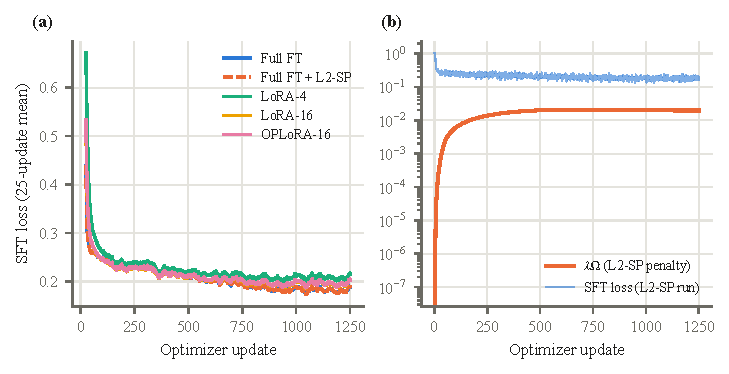
\includegraphics{figures/t1_loss.pdf}
  \caption{SFT loss of the five runs as a 25-update moving average (a), and the L2-SP penalty $\lambda\Omega$ beside the same run's SFT loss on a log scale (b).}
  \label{fig:t1}
\end{figure}

\paragraph{Neither the relative update size $\eta$ nor the subspace interference $\rho_k$ explained the retention differences.}
\citet{oplora} report that updates concentrated in the dominant singular directions forget more, so we expected Full FT, the only method that lost HellaSwag accuracy, to show larger or more concentrated updates. Every unconstrained update had $\rho_k$ of 0.11 to 0.15, near the random level of 0.125 (\Cref{tab:t1diag}), so no method concentrated on the dominant directions. In layers 0 and 13, LoRA-16 changed down\_proj by as much as Full FT relative to $W_0$, yet kept HellaSwag while Full FT lost accuracy, so update size did not predict forgetting either. In these layers both updates corrected GSM8K activations 1.8 to 2.3$\times$ more than HellaSwag contexts and changed the HellaSwag outputs by 2.5 to 3.1\% (\Cref{tab:t1diag}), so the two methods were equally selective for mathematical inputs. In layer 27 both corrected HellaSwag contexts more, and Full FT shifted them by 2.8\% against 1.4\% for LoRA-16 (\Cref{tab:t1diag}). Only the last layer separates the two methods, and the rest of the difference plausibly lies in the embeddings, normalization weights and other matrices that only Full FT updates. These diagnostics apply one layer's change to inputs from the starting model, so they cannot show what caused forgetting.

\begin{table}[t]
  \centering
  \caption{Weight and activation diagnostics for down\_proj, listed as layer 0 / 13 / 27. $R$ is the mean activation correction over 32 GSM8K (math) and 32 HellaSwag (non-math) probe prompts.}
  \label{tab:t1diag}
  \tablebody{tables/t1_diagnostics.tex}
\end{table}

\paragraph{Adapters saved memory and storage but not training time.}
LoRA trains fewer parameters than full fine-tuning \citep{lora}, so we expected adapters to cost less training time, memory and storage. On one T4 GPU, Full FT, L2-SP and both LoRA runs each trained for 2.4 to 2.5 hours (Appendix~\Cref{tab:t1res}). Every method runs the forward pass and backpropagates through the whole network, because the adapters sit inside every layer. Freezing a weight skips only its own gradient and optimizer update. LoRA-16 trained 1.7\% of the parameters, so it stored no gradients or AdamW states for the rest. This cut peak memory to 5.2 GB compared to 13.9 GB for Full FT, and final checkpoint size to 40 MB compared to 2.38 GB for Full FT. L2-SP's overhead was a stored copy of $\theta_0$, and OPLoRA added 40\% training time because our implementation recomputed the projected factors in every forward pass. LoRA-16 therefore reached 91\% of Full FT's math gain with no retention loss at 37\% of its peak memory.

\paragraph{Full fine-tuning inserted MetaMathQA's closing line and repetition loops into unrelated conversations.}
Fine-tuning on one narrow domain can change how a model answers unrelated questions \citep{emergent}, and every MetaMathQA response ends with ``The answer is'', so we expected that closing line to transfer. We annotated 42 greedy responses (two everyday questions in plain, JSON and template formats, 512-token cap) blind to the condition. The three full fine-tuning checkpoints produced 2.7$\times$ as many unnecessary mathematical closings as the three adapters (8 against 3) and 5$\times$ as many repeated passages (5 against 1), while the baseline produced neither (Appendix~\Cref{tab:t1qual}). On one everyday question all three full fine-tuning checkpoints repeated a sentence until the cap (Appendix~\ref{app:t1}). A model trained to end every response with a stated answer appears to add that line where it does not fit, or, with no number to report, to repeat a sentence instead of ending its turn. The likelihood benchmarks never let the model generate, so they cannot register either change, and L2-SP recovered BoolQ while still producing both the closing line and the loop.

\section{Visual Grounding in a Modular Vision-Language Model}
\label{sec:t2}
\subsection{Setup}
\paragraph{Architecture.} SigLIP-base \citep{siglip} encodes each image into 196 patch features $F(I)\in\mathbb R^{196\times768}$, a two-layer MLP connector $g_\phi$ maps each patch into the 1,024-dimensional input space of Qwen3-0.6B \citep{qwen3}, and the visual tokens $Z(I)=s\,g_\phi(F(I))$, with a fixed scale $s$ (Appendix~\ref{app:t2}), replace 196 placeholder tokens in the user turn before the question.

\paragraph{Measuring image use.} A complementary pair applies one question to two images with different answers \citep{vqav2}, so the question alone cannot answer both. We measure image use by replacing the image with the partner image, an unrelated image from the same test set, or no image. All conditions are scored against the original references, and the image-swap penalty is
\begin{equation*}
\Delta_{\mathrm{NLL}}=\mathrm{NLL}(y\mid q,I_{\mathrm{partner}})-\mathrm{NLL}(y\mid q,I_{\mathrm{correct}}),
\end{equation*}
where $\mathrm{NLL}$ is the mean per-token negative log-likelihood, in nats (natural-logarithm units), of the reference answer $y$ to question $q$. It is computed with teacher forcing, i.e.\ each answer token is predicted from the preceding reference tokens.

\paragraph{Curriculum.} Stage 1 trained the connector on 18,000 COCO captions \citep{coco} for 2,250 updates. Stage 2 added LoRA on the attention projections and trained 1,500 updates on annotation-derived pairs, i.e.\ template questions generated from COCO object labels that ask whether an object is present (``Does this image contain [object]?'') or how many there are (1 to 4). Stage 2 also used caption replay, mixing Stage 1 caption examples into training so that captioning is kept. Stage 3 trained 750 updates on natural VQAv2 pairs with replay of captions and annotation-derived pairs.

\paragraph{Scoring.} We report 64 annotation-derived and 96 natural test pairs. Annotation-derived answers are scored by normalized exact match and natural answers by VQA soft accuracy against ten human answers (Appendix~\ref{app:t2}). Pair accuracy requires answering correctly on both images of a pair, and the correct-image advantage is the accuracy drop caused by swapping in the partner image.

\subsection{Results and Analysis}
\paragraph{Answers depended on the image only after training on question-answer pairs.}
\citet{llava} train the connector on captions first so that visual features match the input distribution of the language model, and we expected this alignment to make the image informative for questions as well. During Stage 1 the swap penalty stayed within 0.3 nats of zero on both test sets (\Cref{fig:t2}c). In the same stage the reference answers were less likely with an image than without one (\Cref{fig:t2}b), because the connector had learned the caption distribution and an image steered the frozen model toward a description instead of a short answer. The annotation-derived penalty reached 2.82 nats within the first 250 updates of Stage 2 (\Cref{fig:t2}c), since LoRA and the connector now fitted answers that change with the image. Stage 3 lowered the development NLL of natural questions by 0.59 nats with the image and 0.65 nats without it, and lowered the swap penalty (\Cref{fig:t2}b,c), so natural VQAv2 training improved what the question alone predicts at least as much as it improved image use. Replay held the caption loss at 2.36 after Stage 1 (\Cref{fig:t2}a).

\begin{figure}[t]
  \centering
  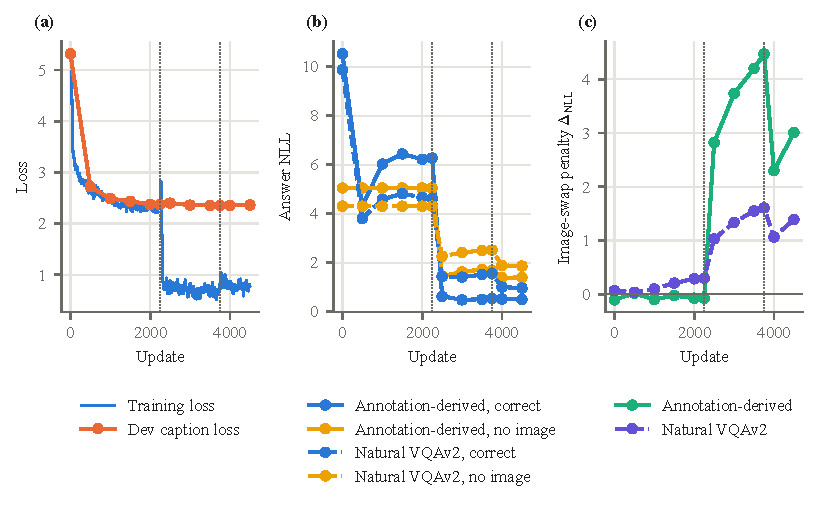
\includegraphics{figures/t2_curves.pdf}
  \caption{Training and development caption loss (a), reference-answer NLL with and without the image (b), and the image-swap penalty $\Delta_{\mathrm{NLL}}$ (c). Dotted lines mark the stage boundaries.}
  \label{fig:t2}
\end{figure}

\paragraph{Annotation-derived answers followed the image, while natural answers often stayed the same for both images.}
Complementary pairs test whether this image dependence follows the evidence, since a model answering from the question's wording alone cannot get both images right \citep{vqav2}. A grounded model should therefore lose accuracy under the swap and give the partner image's answer instead. On annotation-derived questions the swap cut accuracy from 65.6\% to 18.8\% (\Cref{tab:t2}), and the partner-match rate, the share of swapped answers equal to the partner image's reference, was also 65.6\%, so the model read presence and counts from the image in front of it. Counting reached 40.6\% against 90.6\% for presence (Appendix~\Cref{tab:t2full}), consistent with a count needing several separate instances rather than one detected object. On natural VQAv2 the correct-image advantage was 16.2 pp against 46.9 pp for annotation-derived questions (pair-bootstrap intervals in Appendix~\Cref{tab:t2full}), because the model gave one answer to both images in 62.5\% of natural pairs. An answer from the language prior, i.e.\ what the wording alone predicts, is right for at most one image of a pair, which held natural pair accuracy at 13.5\% (\Cref{tab:t2}).

\begin{table}[t]
  \centering
  \caption{Final-test accuracy (normalized exact match for annotation-derived pairs, VQA soft accuracy for VQAv2), pair accuracy and reference NLL under four image conditions.}
  \label{tab:t2}
  \tablebody{tables/t2_main.tex}
\end{table}

\paragraph{Reference likelihood showed image use that greedy generation did not.}
The swap penalty scores the reference answer by teacher-forced likelihood, whereas accuracy scores the top-ranked generated answer, so the two need not agree on whether the image is used. The correct image lowered the test reference NLL on VQAv2 by 0.72 nats, with an interval that excludes zero (Appendix~\Cref{tab:t2full}), yet generation gave one answer to both images in 62.5\% of natural pairs, because raising the reference's probability does not make it the top-ranked answer. On VQAv2, no image scored 36.3\% against 27.9\% for an unrelated image at equal reference NLL (\Cref{tab:t2}), so a wrong image misled generation more than it lowered the likelihood of the right answer. Appendix~\ref{app:t2pairs} shows one pair for each case.

\paragraph{The 196 visual tokens doubled the generation time per answer.}
A frozen FP16 backbone needs no optimizer state, so training cost scales with the trainable connector and adapters. Stage 1 trained 1.84 M connector parameters and Stages 2--3 trained 6.42 M with LoRA, at a peak of 1.67 GB on one T4 GPU, after a one-off feature-caching pass over 9,387 images (Appendix~\Cref{tab:t2res}). Generation took 37 ms with an image against 18 ms without, as the 196 visual tokens dominate the prompt.

\section{Test-Time Compute}
\label{sec:t3}
\subsection{Setup}
\paragraph{Selection rules.} Repeated sampling draws $N$ independent rollouts, i.e.\ complete sampled responses, and a selection rule must recognize a correct one. Rollouts without an extractable answer form one missing-answer group that still votes and is always graded wrong. FirstAns selects the initial rollout, self-consistency takes the majority vote \citep{selfconsistency}, and highest-score selection returns the rollout with the highest quality score (defined below). Rank-weighted consensus (RWC) weights each rollout's vote by its quality rank $r_i$, assigning weight $w_i=(N-r_i)/(N-1)$ and returning $\hat a=\arg\max_a\sum_{i:a_i=a}w_i$.

\paragraph{Quality scores.} The quality scores are the mean sampled-token log-probability $L_i$, i.e.\ how probable the model found its own sampled tokens, and self-certainty
\begin{equation*}
K_i=\frac1{T_i}\sum_{t=1}^{T_i}D_{\mathrm{KL}}\big(U\,\Vert\,p_{i,t}\big),
\end{equation*}
the mean Kullback--Leibler (KL) divergence of each next-token distribution $p_{i,t}$ of the $T_i$-token rollout from the uniform distribution $U$ over the vocabulary \citep{selfcertainty}. It is 0 when every token is equally likely and grows as the model concentrates probability on fewer tokens. For the VLM we also use the visual engagement $V_i$, the mean over tokens of the share $v_{i,t}$ of attention placed on the image, and VisConf $Z_i=V_iC_i$, where $C_i$ is the mean of a per-token certainty $c_{i,t}\in[0,1]$ \citep{visconf} (Appendix~\ref{app:t3defs}).

\paragraph{Protocol.} Oracle coverage, the fraction of questions with at least one correct rollout, bounds every selector. We used 32 supplied rollouts per question from Qwen2.5-3B-Instruct \citep{qwen25} on 1,000 MATH problems \citep{math} and Qwen2.5-VL-3B-Instruct on 1,000 MathVista questions \citep{mathvista}, and report the 800 held-out questions per dataset. Each budget $N$ uses the first $N$ rollouts of ten seeded random orderings of the 32, averaged within and then across questions.

\subsection{Results and Analysis}
\paragraph{Self-consistency missed available correct answers more often than sampling failed to produce one.}
\citet{selfconsistency} show that voting over more sampled reasoning paths raises accuracy, and we expected the gain to follow oracle coverage. On MATH, coverage reached 91.4\% at $N=32$ while self-consistency levelled off at 73.8\% (\Cref{fig:t3sel}a). Averaged over the ten orderings at $N=32$, 17.6\% of questions had a correct rollout that self-consistency missed, against 8.6\% with no correct rollout (Appendix~\Cref{tab:t3fail}). Each added rollout mostly repeated an existing answer and occasionally added a new wrong one, so the number of distinct answers per question tripled from $N=4$ to $N=32$ without changing which answer led the vote. MathVista showed a larger gap between coverage and self-consistency (\Cref{fig:t3sel}b) as its lower per-rollout accuracy, 54.3\% against 66.3\%, left the correct answer in the minority more often. Even the best selector, self-certainty with RWC, stayed 15.9 pp below coverage on MATH.

\begin{figure}[t]
  \centering
  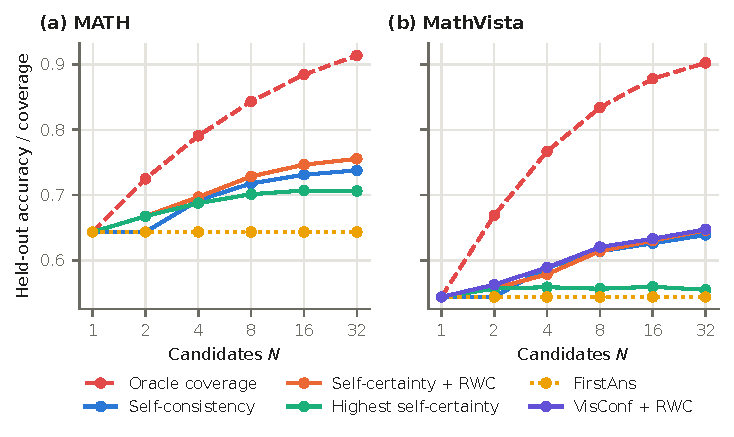
\includegraphics{figures/t3_selection.pdf}
  \caption{Held-out accuracy and oracle coverage against the rollout budget $N$, averaged over ten rollout orders. The distance between coverage and each selector is its selection failure rate.}
  \label{fig:t3sel}
\end{figure}

\paragraph{Self-certainty raised accuracy as an RWC vote weight and lowered it as a single-rollout selector.}
A better selector could close part of this gap. \citet{selfcertainty} report that mean log-probability rises with response length while self-certainty stays nearly length-invariant, and \citet{visconf} report that weighting votes by quality rank outperforms both plain voting and single-rollout selection. At $N=32$ on MATH, self-certainty with RWC beat self-consistency by 1.8 pp with an interval that excludes zero, whereas picking the single most self-certain rollout fell 3.2 pp below it (\Cref{tab:t3}). A vote weight only shifts support among answers that already have votes, so one wrongly top-ranked rollout cannot decide the answer, while a single-rollout selector returns exactly that rollout. Highest mean log-probability fell 9.8 pp below because it ranked a question's long rollouts highest (Appendix~\Cref{tab:t3sig}), and long rollouts were less often correct, as repeated or capped text keeps a high per-token probability.

\paragraph{Visual engagement largely encoded rollout length.}
\citet{visconf} add visual engagement to confidence on the premise that a rollout attending to the image reasons from it, and report a 1.3 pp gain over self-consistency for this model and dataset at $N=32$. On MathVista, VisConf with RWC gained 0.8 pp, but its interval includes zero (\Cref{tab:t3}). Visual engagement correlated with rollout length at a mean within-question Spearman of $-0.69$ (\Cref{tab:t3sig}) because attention to the image falls as the generated text grows, so $V_i$ largely encodes brevity. Tokenwise fusion $Z^{\mathrm{token}}_i$ averages $c_{i,t}v_{i,t}$ over tokens instead of multiplying the rollout means, so $Z^{\mathrm{token}}_i-Z_i=\mathrm{Cov}_t(c_{i,t},v_{i,t})$, the covariance of the two within a rollout. That covariance was negative, with a mean Pearson correlation of $-0.21$ over 800 questions, and tokenwise fusion changed RWC accuracy by $-0.4$ pp (\Cref{tab:t3}). In the cases of Appendix~\ref{app:t3cases}, VisConf with RWC recovered a correct minority answer where self-consistency returned the missing-answer group.

\begin{table}[t]
  \centering
  \caption{Held-out accuracy (\%) at 8 and 32 rollouts, and the difference from self-consistency at 32 with a 95\% paired bootstrap interval.}
  \label{tab:t3}
  \tablebody{tables/t3_methods.tex}
\end{table}

\paragraph{Sequential refinement completed truncated attempts.}
\citet{selfrefine} report that self-revision gains little on math word problems (0 to 0.2 pp) because the model rarely detects its own errors. Under an equal token budget of 3,072 on 50 MATH questions, sequential refinement reached 66\% accuracy, against 62\% for three parallel 1,024-token rollouts and 58\% for one long response (Appendix~\Cref{tab:t3live}). The revision kept the initial answer in 45 of 50 questions and never changed a correct answer, and both of its corrections completed an initial response that had been truncated before giving an answer. Its gain therefore came from extra length and not from detecting errors (Appendix~\ref{app:t3cases}). Equal token budgets came with unequal costs, as the parallel rollouts generated 3.1$\times$ the output tokens of the long response, which never reached its cap. Two to four questions separate the three strategies, so the comparison does not rank them.

\paragraph{Agreement-based stopping halved the cost of 32 rollouts.}
Adaptive-Consistency stops sampling once the revealed answers agree and reports 3.3$\times$ fewer samples at under 0.1 pp of accuracy \citep{adaptiveconsistency}. Our agreement controller stops after 4, 8 or 16 rollouts once one answer leads with at least a fraction $\tau$ of them, and returns the self-consistency answer (Appendix~\ref{app:t3}). With its threshold $\tau=0.625$ selected on the development questions, the agreement controller came within 0.2 pp of 32 rollouts on held-out MATH at 47\% of the generated tokens (Appendix~\Cref{fig:t3cost}a and \Cref{tab:t3adapt}). Of its wrong early stops, 7.7\% would have been corrected by 32 rollouts, because an early wrong majority usually stays the majority (Appendix~\ref{app:t3cases}). On MathVista it stayed within 0.9 pp of 32 rollouts at 33\% of the cost (Appendix~\Cref{fig:t3cost}b), and both controllers lay above the fixed-budget curve at equal cost, since they stop once a vote is settled and keep sampling on contested ones.

\section{Conclusion}
\label{sec:conclusion}

In each experiment the result followed from which outputs the loss or the selection rule measured. Supervised fine-tuning imitates every token of its targets, so the full fine-tuning checkpoints, L2-SP included, learned MetaMathQA's answer template along with its arithmetic. Caption targets taught the VLM connector to elicit descriptions, and the image changed the answers once the training answers changed with it. Consensus and confidence can only choose among the answers the model produces, so they could not recover a correct answer that a minority of rollouts gave.

\bibliographystyle{plainnat}
\bibliography{ref}

\appendix
\section{Experimental Setup: Precision, Leakage Guards and Deviations}
\label{app:dev}

\paragraph{Mixed Precision}
Training used FP16 mixed precision, i.e.\ 16-bit forward and backward passes with the loss scaled up so that small gradients do not round to zero, while the optimizer updated 32-bit copies of the trainable weights. These were all weights for Full FT and Full FT + L2-SP and only the adapters, on a frozen 16-bit backbone, for LoRA and OPLoRA.

\paragraph{Leakage Guards}
MetaMathQA examples matching a GSM8K test question were excluded, and the probe prompts and annotated questions were fixed before any evaluation. VLM development and test images come from COCO val2014 and are disjoint from every training and replay image. Stopping thresholds were selected on 200 development questions and frozen before any of the 800 held-out questions was scored.
\paragraph{Deviations}
The optional 49-token VLM variant was not run. Merged adapters were checked against unmerged ones in FP32 and then required 99.5\% top-1 agreement after the FP16 cast. Annotation-derived VLM labels were checked with fixed area rules instead of viewing each image, and MATH answer pairs whose symbolic comparison timed out count as different answers.

\section{Language Model Fine-Tuning: Supplementary Results}
\label{app:t1}

\paragraph{Benchmark Scores}
\Cref{tab:t1full} adds the raw accuracy of HellaSwag and ARC-Easy, which sums answer log-probabilities without dividing by answer length, to the normalized scores of \Cref{tab:t1}. On ARC-Easy both versions rose for every condition. On HellaSwag the full fine-tuning checkpoints lost less raw accuracy (0.6 pp at most) than normalized accuracy, and L2-SP's raw accuracy stayed at the baseline, so part of the HellaSwag loss comes from how fine-tuning changed the per-character likelihood of long and short endings.

\begin{table}[H]
  \centering
  \caption{Primary and raw accuracy (\%) for the seven evaluation conditions.}
  \label{tab:t1full}
  \apptable{tables/t1_bench_full.tex}
\end{table}

\paragraph{Training Cost}
\Cref{tab:t1res} gives the cost comparison behind the cost paragraph of \Cref{sec:t1}, with the full-model displacement used in the L2-SP comparison. All five runs used one T4 GPU. A resume checkpoint holds the trainable weights with their AdamW states, which is why it is 3$\times$ the final checkpoint. L2-SP kept its 2.4 GB copy of $\theta_0$ in pinned CPU memory and spent 485 s streaming it to the GPU, and OPLoRA spent 31 s on the singular value decompositions of its 196 adapted matrices and stored 323 MB of bases.

\begin{table}[H]
  \centering
  \caption{Trainable parameters, training time, peak GPU memory, checkpoint sizes, final displacement from $\theta_0$ and method-specific overhead for the five runs.}
  \label{tab:t1res}
  \apptable{tables/t1_resources.tex}
\end{table}

\paragraph{BoolQ Answer Bias}
\Cref{tab:t1bool} splits BoolQ accuracy by the gold answer, since a two-option likelihood test also moves with the model's preference for one answer word. 62.2\% of BoolQ questions have the gold answer ``yes''. Full FT gained on ``no'' questions and lost more on ``yes'' questions, whereas LoRA-16 improved on both.

\begin{table}[H]
  \centering
  \caption{Share of BoolQ questions answered ``yes'' and accuracy (\%) on the questions whose gold answer is ``yes'' or ``no''.}
  \label{tab:t1bool}
  \apptable{tables/t1_boolq.tex}
\end{table}

\paragraph{Qualitative Annotation}
\Cref{tab:t1qual} counts the flags over the six annotated responses of each condition (two questions in plain, JSON and template formats). The seven responses to each prompt were read in a shuffled order with the condition hidden. A response violates the format if a JSON answer is not one JSON object or a template field is left unfilled. It is incoherent if it does not answer the prompt, for example by repeating the offer back, and it repeats if one sentence or clause loops. It has mathematical framing if it adds a solution-style answer line, and it is truncated if it reaches the 512-token cap. The baseline itself repeated the wish offer back in the plain and JSON formats and left the wish template unfilled, and only one of the seven JSON answers to the second question was valid JSON.

The excerpt comes from one of the two (question, format) cells whose flags differed most across the seven conditions, a rule fixed before reading. In one of the two cells whose flags differed most, all three full fine-tuning checkpoints repeated one sentence until the cap on ``I've had enough of my husband. What should I do?'', while the baseline and the adapters answered in under 90 tokens.
\begin{table}[H]
  \centering
  \caption{Annotation flags per condition over six responses each. No response was flagged as inappropriate.}
  \label{tab:t1qual}
  \apptable{tables/t1_qual.tex}
\end{table}


\section{Visual Grounding: Supplementary Results}
\label{app:t2}

\paragraph{Connector Scale}
The fixed scale $s=0.0546$ matches the mean norm of the visual tokens to that of Qwen's text embeddings on the training captions, so the visual tokens enter the frozen model at the size of word embeddings.
\paragraph{Answer Scoring}
Annotation-derived answers are scored by normalized exact match, i.e.\ equality after lowercasing, removing punctuation and articles and writing numbers as digits. VQAv2 answers are scored by VQA soft accuracy, the mean over the ten ways of leaving out one human answer of $\min(1,m/3)$, where $m$ counts the remaining nine answers that match, so an answer given by four or more annotators scores 1.

\paragraph{Results by Question Type}
\Cref{tab:t2full} breaks the final-test results of \Cref{tab:t2} down by question type, with the pair diagnostics and the correct-image advantages behind the grounding paragraphs of \Cref{sec:t2}.

\begin{table}[H]
  \centering
  \caption{Final-test results by question type and image condition, with 95\% pair-bootstrap intervals for the correct-image advantages over the complementary swap. Counting and open-ended (other) questions had the lowest accuracy.}
  \label{tab:t2full}
  \apptable{tables/t2_final_grounding.tex}\par\medskip
  \apptable{tables/t2_final_vqa.tex}
\end{table}

\paragraph{Illustrative Pairs}
\label{app:t2pairs}
We take the pair with the smallest id in each outcome class, a rule fixed before reading any generation. For ``How many stop signs can you see?'' (references 1 and 3) the model answered 1 and 3, and 3 and 1 after the swap, so its counts followed the image. For ``What color is the couch?'' (references red and black) it answered white with both the correct and the swapped image, a wording-driven answer that lowers natural pair accuracy.
\paragraph{Training Cost}
\Cref{tab:t2res} gives the trainable parameters, time and peak memory per stage behind the cost paragraph of \Cref{sec:t2}.

\begin{table}[H]
  \centering
  \caption{Training cost by stage on one T4 GPU, with the one-off feature caching. The frozen backbone kept peak memory under 1.7 GB.}
  \label{tab:t2res}
  \apptable{tables/t2_resources.tex}
\end{table}

\section{Test-Time Compute: Supplementary Results}
\label{app:t3}
\paragraph{Score Definitions}
\label{app:t3defs}
The visual engagement of token $t$, $v_{i,t}$, is the attention mass on image positions as a share of the mass on image, prompt-text and earlier generated positions, averaged over all heads and the 36 decoder layers. The calibrated certainty $c_{i,t}$ is the token's KL divergence from the uniform distribution $U$, rescaled to $[0,1]$ by the 5th and 95th percentiles over the revealed rollouts of the question \citep{visconf}.

\paragraph{Live Refinement Experiment}
\Cref{tab:t3live} supports the refinement result in \Cref{sec:t3} with accuracy, actual tokens, runtime and truncation for the three strategies. The sequential strategy is charged for the shared initial response and its longer revision prompt.

\begin{table}[H]
  \centering
  \caption{Live comparison on 50 MATH questions with Qwen2.5-3B-Instruct (FP16, batch 1, one T4). Tokens and seconds are per question. Refinement answered the most questions at less output than parallel sampling.}
  \label{tab:t3live}
  \apptable{tables/t3_live.tex}
\end{table}

\paragraph{Failure Decomposition and Signals}
\Cref{tab:t3fail} separates sampling failures from selection failures, and \Cref{tab:t3sig} lists the length and correctness associations of each score.

\begin{table}[H]
  \centering
  \caption{Coverage, sampling failures (no correct rollout) and selection failures (a correct rollout missed), in percent of held-out question orders. Selection failures grow with $N$.}
  \label{tab:t3fail}
  \apptable{tables/t3_failures.tex}
\end{table}

\begin{table}[H]
  \centering
  \caption{Mean within-question Spearman correlation of each score with rollout length, and the correctness difference between each score's top and bottom quartile of rollouts at $N=32$. The vision scores correlate negatively with rollout length.}
  \label{tab:t3sig}
  \apptable{tables/t3_signals.tex}
\end{table}

\paragraph{Adaptive Stopping}
The agreement controller checks after 4, 8 and 16 rollouts and stops when one answer other than the missing-answer group leads alone with at least a fraction $\tau$ of the revealed rollouts, and otherwise draws all 32. \Cref{tab:t3adapt} gives the development-selected thresholds, held-out accuracy, cost and stopping distribution, and \Cref{fig:t3cost} places both controllers on the fixed-budget accuracy--cost curve. The quality controller also requires the RWC answer to be the same as the self-consistency answer and to lead the runner-up by at least a fraction $\gamma$ of the total vote weight, and both controllers return the self-consistency answer.

\begin{figure}[H]
  \centering
  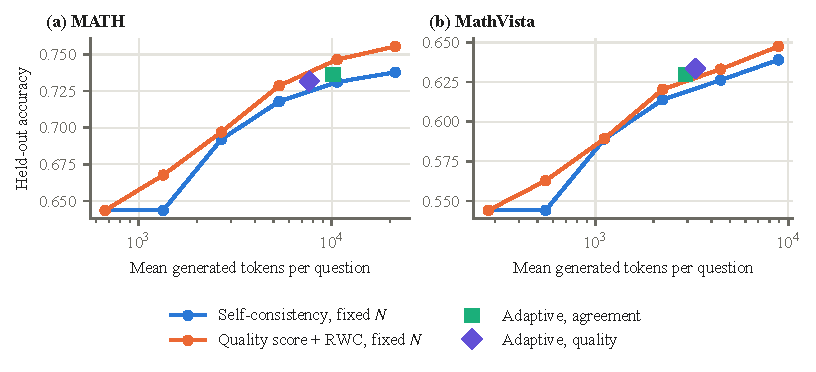
\includegraphics{figures/t3_cost.pdf}
  \caption{Held-out accuracy against mean generated tokens for fixed budgets and the two adaptive controllers. The quality score is self-certainty for MATH and VisConf for MathVista. Adaptive stopping came within 1 pp of 32 rollouts at a third to a half of the tokens.}
  \label{fig:t3cost}
\end{figure}

\begin{table}[H]
  \centering
  \caption{Held-out adaptive stopping with thresholds frozen on the development questions, against fixed budgets. Agreement-based stopping halved the cost of 32 rollouts on MATH at $-0.2$ pp.}
  \label{tab:t3adapt}
  \apptable{tables/t3_adaptive.tex}
\end{table}

\paragraph{Illustrative Cases}
\label{app:t3cases}
For selection we take the smallest held-out question id where self-consistency and the quality-weighted RWC rule disagree at $N=32$ in the first rollout order (self-certainty for MATH, VisConf for MathVista). For refinement we take the first wrong-to-correct revision, and for stopping the first wrong early stop where all 32 rollouts would have voted correctly.
\begin{itemize}
\item \textbf{Selection, MathVista question 10} (gold E, one of 65 disagreements). Ten of the 32 rollouts gave no extractable answer, one of them repeating ``Circle with a diagonal line'' until the cap, so self-consistency returned the missing-answer group. VisConf with RWC returned E, which 8 rollouts gave.
\item \textbf{Selection, MATH test question 531} (gold $-8$, one of 56 disagreements). Self-consistency returned $-11$ from 3 votes, and self-certainty with RWC returned $-11+\sqrt3$ from 2 votes. Both rules were wrong, as the leading answer held only 3 of the 32 votes.
\item \textbf{Refinement, MATH test question 2358} (gold $2\sqrt5$). The 1,024-token first attempt was cut off before giving an answer, and the revision finished the derivation to $\sqrt{20}=2\sqrt5$. No revision changed a correct answer to a wrong one.
\item \textbf{Stopping, MATH test question 1803} (gold $\tfrac35$). The agreement controller stopped after 8 rollouts on $\tfrac45$, while 16 of the 32 rollouts gave $\tfrac35$ and the 32-rollout vote chose it.
\end{itemize}

\end{document}
